\documentclass[11pt]{article}
\usepackage[margin=1in]{geometry}
\usepackage{amsmath,amssymb}
\usepackage{graphicx}
\usepackage{booktabs}
\usepackage{array}
\usepackage{hyperref}
\usepackage{natbib}
\usepackage{authblk}

\title{Empirical Phase Diagrams of Grokking Failure under Data Skew, and a Low-Dose Rescue Intervention}
\author{}
\date{}

\begin{document}
\maketitle

\begin{abstract}
This paper reports an empirical study, not a closed-form theory. We map $(\alpha, \lambda)$ grokkability---data skew against weight decay---on an autoregressive counting task under a finite compute budget of up to $10^6$ steps; the resulting boundary is a finite-budget empirical phase diagram, not evidence of an asymptotic phase transition. The onset of substantial rescue probability lies in the $0.4\%$--$0.8\%$ injected-dose range; a batch/step-fixed, probabilistically-implemented sweep deconfounds this from batch size and update count and shows a gradual rise rather than the sharper jump seen when batch size varies with dose. A controlled ranking of interventions shows that, among those tested, only injection drawn uniformly across the full state space achieves complete rescue. The failure and rescue pattern transfers to a second arithmetic task, modular addition, under sample-count-matched controls. A third, non-arithmetic task, Dyck-1 forced-position prediction, is included as a deliberately harder out-of-domain stress test: it qualifies rather than confirms the transfer claim, reproducing the failure topology and the injection-ranking direction while falling short of complete rescue and budget-monotonic behavior. All findings are reported at $n\le 12$, $d\le 128$ scale.
\end{abstract}

\section{Introduction}

Grokking---the delayed generalization of a model that has already fit its training set---was first reported by \citet{power2022grokking} on small algorithmic datasets, and has since accumulated a broad literature on when and why it occurs \citep{liu2022effectivetheory,liu2022omnigrok,nanda2023progress}. \citet{zhao2026grok} recently sharpened one open question in this literature by studying LARGECOUNTER, an autoregressive binary counting task on which succinct algorithmic circuits provably exist \citep{bergstrasser2026succinct}: does training on a stratified sample---one that over-represents rare carry-chain states---\emph{create} grokking on those states, or merely \emph{extend} an effect that would occur anyway? Zhao's evidence is a single qualitative comparison between uniform and stratified sampling. It leaves the shape of grokkability under continuous data skew, and the minimal intervention needed to rescue a model once it is trapped, entirely uncharacterized.

We answer both questions with the same experimental apparatus. We build a continuous skew axis $\alpha$ (Zipf-weighted minibatch sampling, $P_\alpha(x)\propto(x+1)^{-\alpha}$) crossed against weight decay $\lambda$, and map grokkability across this $(\alpha,\lambda)$ plane on the LARGECOUNTER task. The resulting map exhibits two regimes---a boundary layer where additional compute budget improves outcomes, and a deep-trap interior that does not escape even at four times the originally tested budget. The map's most direct practical payoff is a precise answer to Zhao's rescue question: a low dose of injected examples drawn uniformly across the entire state space, on the order of $0.8\%$ of each minibatch, rescues both failure modes we observe, and among a set of controls varying sample count, targeted rarity, and breadth of the injected examples across the state space, uniform full-state injection is the one that rescues.

Our contributions, in the order we present them, are:
\begin{enumerate}
\item An empirical, finite-budget $(\alpha,\lambda)$ phase diagram with two failure boundaries and a two-regime kinetic/deep-trap structure, reproduced at a second problem size with an exposure-matching protocol that avoids conflating training dynamics with the underlying failure structure (\S\ref{sec:results-map}).
\item A low-dose rescue intervention validated by a controlled comparison ranking sample count, rarity, and distributional breadth against one another (\S\ref{sec:results-rescue}).
\item A family-discrimination analysis of the boundary's shape, evaluated by a pre-specified held-out prediction test (\S\ref{sec:results-family}).
\item A pre-specified local robustness study across width, learning rate, depth, and optimizer choice, with four of seven directional predictions confirmed at both tested boundary cells (\S\ref{sec:results-robustness}), and transfer of the injection-ranking direction to a second arithmetic task, modular addition, under sample-count-matched controls (\S\ref{sec:results-modadd}).
\end{enumerate}

We state our scope precisely because the boundary of what these experiments show is itself informative. The phase diagram we report is empirical and finite-budget: we do not claim an asymptotic phase transition or a critical exponent. The rescue intervention we report is the best-ranked among those we tested, not a proof of necessity. The transfer result we report is to a second \emph{arithmetic} task; a third, non-arithmetic task (Dyck-1 forced-position prediction, \S\ref{sec:results-dyck}) is included precisely to test how far this transfers, and it draws that boundary for us: the failure topology and the direction of the injection ranking reproduce, while complete rescue and budget-monotonic behavior do not.

\section{Related Work}

\textbf{Grokking and its mechanisms.} \citet{power2022grokking} established the toy-algorithmic-task recipe this paper's LARGECOUNTER setup descends from. Subsequent work has proposed a wide range of mechanistic accounts of why grokking occurs: weight-norm dynamics and a ``Goldilocks zone'' between memorization and confusion \citep{liu2022effectivetheory,liu2022omnigrok}; measurable progress proxies tied to Fourier-structured circuits \citep{nanda2023progress}; competing memorizing and generalizing circuits distinguished by parameter efficiency \citep{varma2023circuitefficiency}; group-theoretic representations \citep{chughtai2023toymodel}; a lazy-to-rich training-dynamics transition with rigorous sample-complexity bounds \citep{mohamadi2024whygrok}; an early-versus-late-phase implicit-bias dichotomy under weight decay \citep{lyu2024dichotomy}; complexity and compression measures that rise then fall across training \citep{liu2023grokkingcompression,demoss2024complexitydynamics}; and causal, representation-level precursors to generalization onset \citep{sivasankar2026circuitsync,howe2026representationalpriors}. \citet{demellokoch2025twophase} unify grokking with double descent and the information bottleneck under a shared two-phase timescale structure, echoing the two-regime structure we report in \S\ref{sec:results-map}. We treat this diversity of mechanistic accounts as the backdrop against which our own controlled injection ranking (\S\ref{sec:results-rescue}) should be read: our ranking points to a data-side coverage effect, compatible with, rather than a replacement for, model-side accounts of what happens once training data is fixed.

\textbf{Phase-transition framings.} A parallel line of work treats grokking as a genuine physical phase transition and studies it with tools from statistical mechanics: finite-size scaling and Binder-cumulant crossings against group order \citep{bi2026falsifiable}; effective-dimensionality crossings interpreted as self-organized criticality \citep{wang2026dimensional}; adaptive-kernel feature-learning theory mapped onto first-order phase transitions \citep{rubin2024firstorder}; and spectral-entropy collapse of the representation covariance as a geometric phase-transition signature \citep{truong2026spectralentropy}. Our $(\alpha,\lambda)$ map uses a different, complementary axis---empirical skew and weight decay under a fixed, finite compute budget---and we do not claim the stronger asymptotic or critical-exponent language these works use.

\textbf{Rescuing and accelerating grokking.} Prior interventions to induce or accelerate grokking include knowledge distillation from an already-grokked model on a related distribution \citep{singh2025datafallsshort}; embedding transfer from a weaker model \citep{xu2025letmegrok}; and learned gradient transformations \citep{zhou2025neuralgrok}. These operate on data quantity, initialization, or gradients respectively; our own intervention (\S\ref{sec:results-rescue}) operates directly on the training distribution's support and ranks coverage above quantity or targeted rarity as the more effective lever, among those tested.

\textbf{Weight decay as a modeling choice.} We use AdamW \citep{loshchilov2019decoupled} throughout; its implicit bias differs from that of SGD with momentum \citep{xie2024implicitbias}, which we use as a comparison point in \S\ref{sec:results-robustness}, and its role in grokking's timing has an independent analytic treatment orthogonal to our skew axis \citep{kim2026weightdecayclock}. We also position our own findings against \citet{doshi2023togrok}'s account of what weight decay mechanistically does to memorizing versus generalizing circuits.

\textbf{Data skew and distribution shift.} \citet{carvalho2025grokkingexplained} formalize grokking as arising from a train/test distribution shift induced by controlled imbalanced sub-category sampling---the closest prior formalization of ``skew causes grokking failure''; our continuous-axis phase diagram substantially extends this picture. \citet{zhu2024criticaldatasize} characterize a related but distinct data-quantity axis, formalizing critical-size phase transitions as a function of model size. We further situate our skew protocol within the broader long-tailed learning literature \citep{zhang2021longtailed,dealvis2024longtailsurvey} and the curriculum-learning tradition \citep{bengio2009curriculum}; our finding that broad coverage outperforms targeted rare-example injection (\S\ref{sec:results-rescue}) directly complicates the naive curriculum-learning intuition that rare or difficult examples should be specifically targeted.

\textbf{Task foundations.} The LARGECOUNTER task is grounded in the succinctness result of \citet{bergstrasser2026succinct} and directly reproduces the design of \citet{zhao2026grok}. Our second and third tasks draw on the modular-arithmetic grokking literature \citep{gromov2023grokkingmodular,doshi2024modularpolynomials,doshi2023togrok,mccracken2025universalabstract} and the formal-language-recognition literature establishing Transformers' ability to recognize Dyck languages \citep{weiss2021thinking,ebrahimi2020dyckn,bhattamishra2020ability,yao2021boundedhierarchical,merrill2022saturated,strobl2024survey}.

\section{Setup}

\subsection{Main task: LARGECOUNTER}
We reproduce Zhao's LARGECOUNTER task faithfully: an autoregressive, big-endian binary counter over vocabulary $\{0,1,\#\}$. Each training example is a single transition $x\to x+1$: the input token sequence is $\mathrm{bin}(x)\,\#\,\mathrm{bin}((x+1)\bmod 2^n)$, length $2n+1$, with $x$ the state being sampled under $P_\alpha$; the loss is masked to only the $n$ target-bit positions after \#, so the model is never asked to predict $x$ itself, only the ripple-carry successor. Big-endian order within each $n$-bit half is essential: it makes carry propagation non-local, requiring the model to resolve a low-bit carry before emitting a high-order bit that appears earlier in its own $n$-bit target, which is what creates a genuine grokking delay rather than a trivial two-state transduction. We use a causal decoder-only Transformer \citep{vaswani2017attention} with rotary position embeddings \citep{su2021roformer}, 2 layers, 4 heads, $d=64$ unless otherwise noted, trained with AdamW \citep{loshchilov2019decoupled} (default $\beta=(0.9,0.999)$, no dropout, no gradient clipping) at learning rate $10^{-3}$ with a cosine-annealed schedule over the full step budget, batch size 128, and a $10\times$ multiplicative rescaling of every \texttt{nn.Linear} weight and bias after PyTorch's default initialization (used for LARGECOUNTER and Dyck-1; modular addition, \S\ref{sec:results-modadd}, uses the unscaled default). Evaluation is teacher-forced accuracy over the $n$ target-bit positions per transition (a transition counts as correct only if every target bit matches), not free-running/sampled decoding; $A_{\mathrm{unif}}$ and $A_{\mathrm{hi}}$ average this per-transition accuracy over the $2^n$ possible states $x$. We report results at $n=10$ (1024 states) as the primary setting, with $n=12$ used for an exposure-matched finite-size check.

\subsection{Skew protocol}
We construct a continuous skew axis via frequency-weighted minibatch sampling: each training example is drawn with replacement according to $P_\alpha(x)\propto(x+1)^{-\alpha}$, so $\alpha=0$ is uniform and larger $\alpha$ concentrates training mass on small-$x$ states. Frequency weighting, rather than subset selection at a fixed skewed ratio, is necessary here: under a no-replacement fixed-fraction subset-selection protocol, the trailing-ones (carry-chain) composition of the resulting training set is empirically flat in $\alpha$, because a contiguous low-$x$ block has the same trailing-ones distribution as the full state space. The rarity-vs-frequency mechanism we study exists only under the frequency-weighted protocol.

\subsection{Verdict rule}
We classify every trained model by two population-level accuracies: $A_{\mathrm{unif}}$, whole-sequence accuracy averaged uniformly over the full state space, and $A_{\mathrm{hi}}$, the same accuracy restricted to the highest-weight decile under $P_\alpha$. A run is \textsc{Grok} if $A_{\mathrm{unif}}>0.9$; \textsc{Trap} if $A_{\mathrm{hi}}>0.9$ and $A_{\mathrm{unif}}<0.5$; \textsc{Crush} if $A_{\mathrm{hi}}<0.9$ and $A_{\mathrm{unif}}<0.5$; and \textsc{Partial} otherwise. This rule is frozen prior to the experiments reported here and used unchanged throughout. Moving the $A_{\mathrm{unif}}$ cutoff to $0.85$ or $0.95$ shifts the overall grok fraction on the main grid by at most $6$ percentage points ($0.516$/$0.508$/$0.452$ at cutoffs $0.85$/$0.9$/$0.95$) and the $\alpha=2.5$ ceiling by less than $0.04$, so the qualitative topology is not an artifact of the particular threshold.

\subsection{Exposure-matching protocol}
Comparing training outcomes across problem sizes $n$ requires care: doubling the state space at a fixed step budget halves the average number of times each state is visited, so an apparent boundary shift with $n$ can reflect this exposure change rather than a change in the underlying failure structure. We therefore scale the step budget with $n$ (specifically $2^n$) whenever comparing across problem sizes, and report both exposure-matched and unmatched comparisons where relevant.

\subsection{Second and third tasks}
For modular addition, each example is the length-4 sequence $[a,b,\mathrm{SEP},(a+b)\bmod p]$, vocabulary $p+1$ over $\mathbb{Z}_p\cup\{\mathrm{SEP}\}$ ($p=97$, SEP token id $p$), with loss and accuracy computed only at the final position (predicting $(a+b)\bmod p$ from $a,b,\mathrm{SEP}$); the evaluation population is all $p^2$ operand pairs. We skew operand $a$ under $P_\alpha$ while sampling $b$ uniformly; skewing the combined pair index $a p+b$ instead concentrates $99.95\%$ of probability mass on a single operand value at $\alpha=2.5$ and collapses the task, so we skew a single operand. The targeted injection pools are defined analogously to the counting task's carry-length pools: ``tail'' is the rarest decile of $a$-values (large $a$, matching the direction the skew starves), ``head'' is the most frequent decile (small $a$). The model, optimizer, batch size, and evaluation convention match \S3.1; only the initialization scale differs (\S3.1), $n=4$ (task-specific input width) replaces the counting task's $n$, and the step budget is $20{,}000$ (the modular-addition failure region resolves at this shorter budget; the formal grid of \S\ref{sec:results-modadd} and Figure~\ref{fig:modadd} uses it throughout). For our third task, we use sequence length $L=10$ ($C_{10}=16{,}796$ valid Dyck-1 paths of 10 pairs, 20 bracket tokens), the same model/optimizer/batch-size/evaluation convention as \S3.1 with a $60{,}000$-step budget (matching LARGECOUNTER's primary budget; \S\ref{sec:results-dyck}'s trajectory comparison additionally uses $240{,}000$ steps), and pose \emph{forced-position next-token prediction} rather than open-vocabulary string recognition: at each position, the input prefix under the Dyck-1 grammar is deterministic (forced open at depth $0$, forced close when the remaining length equals the current depth) at exactly the positions used for scoring, and free (either bracket keeps the path completable) elsewhere; loss and accuracy are computed only at forced positions, so getting a forced prediction wrong is the error signal a recognizer would otherwise get from an invalid string. We skew training frequency by each path's maximum nesting depth $m(\pi)$, $P_\alpha(\pi)\propto(\mathrm{rank}(m(\pi))+1)^{-\alpha}$ where $\mathrm{rank}$ orders paths ascending by $m(\pi)$ (shallow/common paths get low rank, deep/rare paths get high rank)---the Dyck-1 analogue of carry-chain length, since deep paths require longer-range tracking of nesting state. The targeted injection pools are the shallowest quintile of paths by max depth (``head'') and the deepest quintile (``tail''). As in \S3.2, we use a frozen four-way verdict rule with $A_{\mathrm{unif}}$ computed over the full enumerated path set and $A_{\mathrm{hi}}$ over its highest-weight decile under $P_\alpha$.

\subsection{Preregistration}
Two analyses in this paper were committed to before the corresponding data were collected, with the commitment recorded by file timestamp: predictions for eight held-out $\alpha$ values from the family-discrimination fit (\S\ref{sec:results-family}), and seven directional robustness predictions plus two additivity-test cells (\S\ref{sec:results-robustness}). We use ``pre-specified'' rather than ``preregistered'' throughout, since a filesystem timestamp is evidence of pre-data specification but not registry-grade provenance.

\subsection{Compute}
The full experimental program, including exploratory pilots that informed later confirmatory grid design, totals approximately 130 GPU-hours on a single consumer GPU (RTX 5080).

\section{Results}

\subsection{The $(\alpha,\lambda)$ phase diagram and its kinetics}
\label{sec:results-map}

Figure~\ref{fig:phasediagram} maps grokkability across weight decay $\lambda\in[0.05,0.5]$ (with $\alpha\le1.5$ additionally probed up to $\lambda=1.0$ to bracket the wider channel at low skew) and skew $\alpha\in[0,3]$ at $n=10$. The grok-channel weight-decay ceiling decreases monotonically with $\alpha$: bootstrapped 90\% intervals place the ceiling at $0.764$ ($[0.703,0.851]$, resolved within the extended $\lambda\le1.0$ probe) at $\alpha=1.5$, falling to $0.305$ ($[0.302,0.401]$) at $\alpha=2.0$, $0.190$ at $\alpha=2.1$, $0.123$ at $\alpha=2.25$, and $0.051$ ($[0.044,0.060]$) at $\alpha=2.7$, beyond which no tested weight decay down to $0.02$ rescues generalization. A grid refined by a factor of roughly three around this boundary yields ceiling estimates statistically consistent with the coarser grid at every shared $\alpha$ (Table~\ref{tab:gridconvergence}), so this near-vertical right edge is a property of the task, not an artifact of grid coarseness.

Each cell is 3--5 seeds; ceilings are the linear interpolation of mean $A_{\mathrm{unif}}$ across the $\lambda$ grid crossing the $0.9$ threshold, and 90\% intervals are the 5th/95th percentiles of $2{,}000$ seed-level bootstrap resamples of that interpolation (Appendix~A gives the full per-cell seed counts).

\begin{figure}[t]
\centering
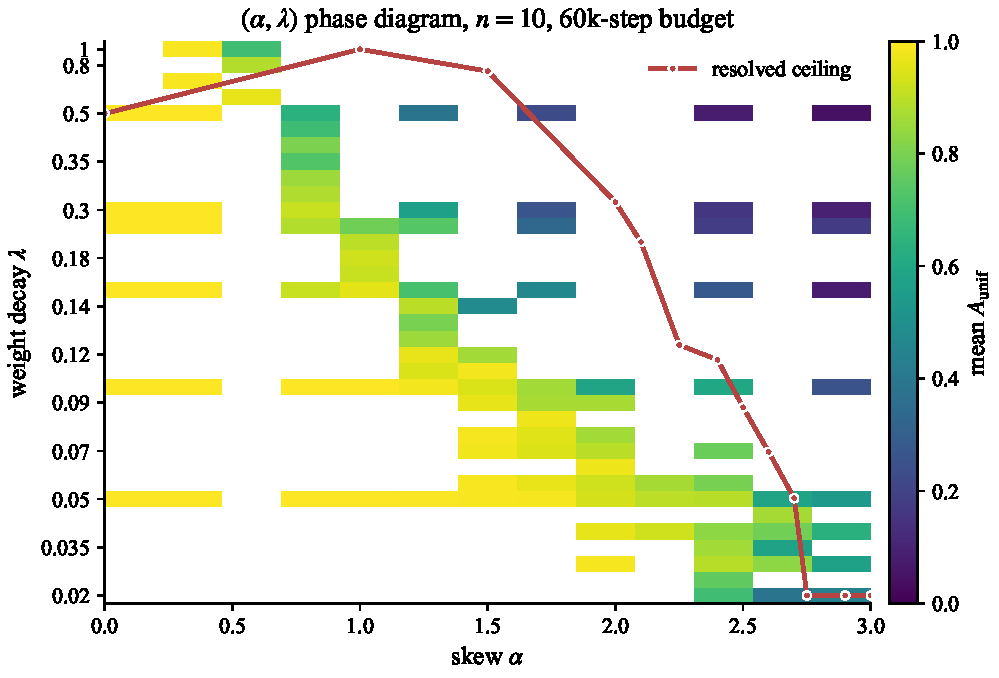
\includegraphics[width=0.85\textwidth]{fig1_phasediagram.pdf}
\caption{The $(\alpha,\lambda)$ phase diagram at $n=10$, 60{,}000-step budget. Color encodes mean $A_{\mathrm{unif}}$ per cell; the red curve traces the resolved weight-decay ceiling.}
\label{fig:phasediagram}
\end{figure}

\begin{table}[t]
\centering
\caption{Grid-resolution convergence: sparse pilot grid vs. densified grid ceiling estimates ($n=10$, 60k budget). Estimates agree within the interpolation tolerance at every shared $\alpha$.}
\label{tab:gridconvergence}
\begin{tabular}{lccc}
\toprule
$\alpha$ & Sparse-grid ceiling & Dense-grid ceiling & \# points (sparse / dense) \\
\midrule
2.0  & $0.305$ & $0.305$ & 9 / 11 \\
2.25 & $0.124$ & $0.123$ & 10 / 11 \\
2.5  & $0.086$ & $0.089$ & 10 / 11 \\
2.75 & $<0.030$ & $<0.020$ & 10 / 13 \\
2.9  & $<0.020$ & $<0.020$ & 4 / 6 \\
3.0  & $<0.020$ & $<0.020$ & 9 / 9 \\
\bottomrule
\end{tabular}
\end{table}

The diagram exhibits two regimes. Near the boundary, additional compute budget measurably improves outcomes: three cells sampled at both 60{,}000 and 240{,}000 steps each show higher mean accuracy at the longer budget, with one cell reaching full generalization at the extended budget from a partial state at the shorter one. Each budget uses its own cosine-annealed schedule over its full length (\S3.1), so the 60k and 240k runs are two independently-scheduled training protocols rather than the same trajectory observed at two checkpoints; we interpret the budget comparisons accordingly. Deep in the interior, at $\alpha=2.25$ and $\alpha=2.5$ with $\lambda=0.3$, extending training to $10^6$ steps---four times our previously tested extended budget---does not rescue generalization in any of eight runs (accuracy range $0.35$--$0.80$, with no upward trend against budget). Repeating the full grid at $n=12$ under our exposure-matching protocol (Table~\ref{tab:n12grid}) reproduces this structure, with the ceiling at $\alpha=2.0$ falling by a factor of $1.42$ relative to $n=10$, ruling out an $n=10$-specific artifact.

\begin{table}[t]
\centering
\small
\caption{$n=12$ exposure-matched grid (mean $A_{\mathrm{unif}}$, 3 seeds/cell, 240{,}000-step budget), the full grid underlying the $n=12$ replication.}
\label{tab:n12grid}
\begin{tabular}{lcccccc}
\toprule
$\alpha$ & $\lambda{=}0.05$ & $0.1$ & $0.15$ & $0.2$ & $0.3$ & $0.5$ \\
\midrule
0.0 & 1.00 & 1.00 & 1.00 & 1.00 & 1.00 & 1.00 \\
1.0 & 1.00 & 1.00 & 1.00 & 1.00 & 1.00 & 1.00 \\
2.0 & 0.99 & 0.99 & 0.91 & 0.91 & 0.80 & 0.53 \\
2.25 & 0.98 & 0.96 & 0.60 & 0.60 & 0.33 & 0.23 \\
2.5 & 0.88 & 0.67 & 0.36 & 0.24 & 0.16 & 0.08 \\
2.75 & 0.52 & 0.29 & 0.12 & 0.09 & 0.10 & 0.02 \\
3.0 & 0.21 & 0.11 & 0.08 & 0.05 & 0.03 & 0.01 \\
\bottomrule
\end{tabular}
\end{table}

The same boundary is accompanied by a kinetic signature. At fixed $\lambda=0.3$, the fraction of runs that have not generalized after 240{,}000 steps rises monotonically across fifteen seeds per cell: $0\%$ at $\alpha\le 2.0$, $27\%$ at $\alpha=2.1$, $53\%$ at $\alpha=2.2$, and $60\%$ at $\alpha=2.25$ (Figure~\ref{fig:kinetics}). At the lower weight decay $\lambda=0.05$, where every seed eventually generalizes within budget, the median time to generalization rises from $12{,}000$ steps at $\alpha=2.0$ to $171{,}250$ steps at $\alpha=2.75$. We describe this as critical-slowing-like behavior---a monotonic rise in failure probability and generalization time approaching the boundary---without claiming a proven divergence or a critical exponent.

\begin{figure}[t]
\centering
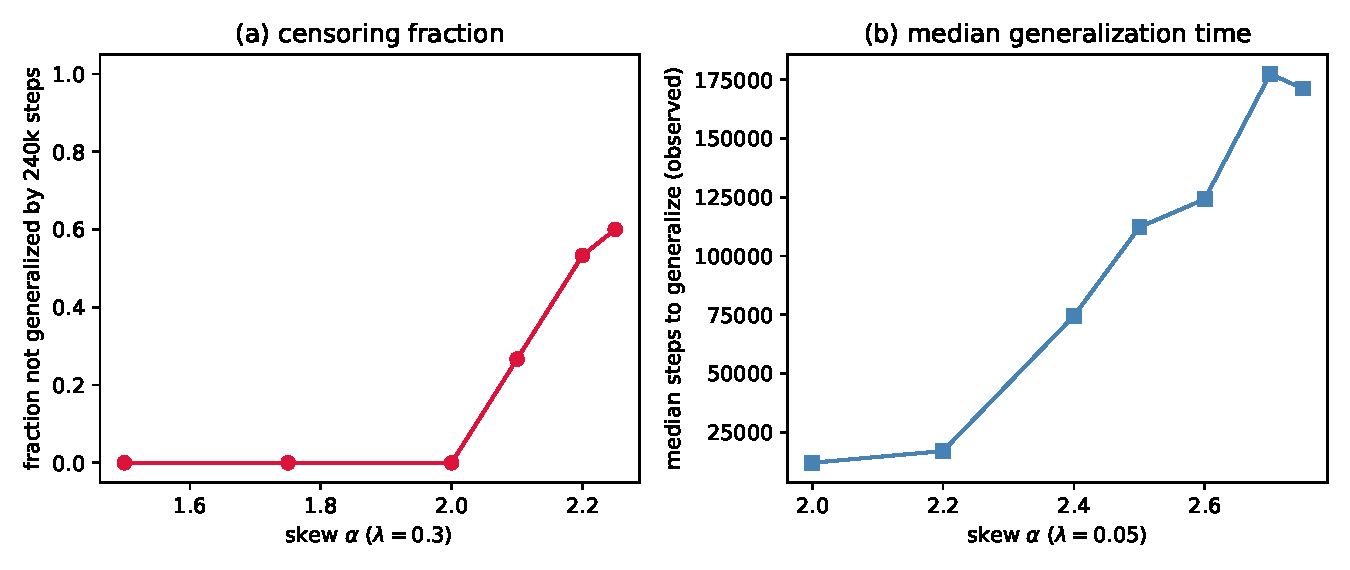
\includegraphics[width=0.95\textwidth]{fig2_kinetics.pdf}
\caption{Kinetic signature of the boundary. (a) Censoring fraction (fraction not generalized by 240k steps), $\lambda=0.3$, 15 seeds/cell. (b) Median generalization time (observed seeds only), $\lambda=0.05$.}
\label{fig:kinetics}
\end{figure}

\subsection{A low-dose rescue intervention}
\label{sec:results-rescue}

Injecting a small fraction of uniformly-sampled examples into an otherwise skewed minibatch rescues both failure modes identified by the verdict rule: \textsc{Trap} (accuracy is high on the frequent head but low overall---``trapped'' on the head) and \textsc{Crush} (accuracy is low even on the head---``starved'' of any learnable signal). Doses below $0.78\%$ ($k=1$ per 128) were initially implemented by holding $k=1$ fixed and varying batch size (1024, 512, 256, 128) with step count scaled inversely to hold total sample count fixed; this protocol varies batch size and optimizer-update count jointly with dose. To deconfound dose from batch size and update count, we separately ran a second dose sweep with batch size (128) and step count ($60{,}000$) held fixed throughout: at each step, with probability $q$ one of the 128 slots is replaced by a uniformly-sampled state, giving expected dose $q/128$; $q=1$ exactly reproduces the batch-128 endpoint of the first sweep. Across $q\in\{0.1,0.25,0.5,0.75,1.0\}$ (expected dose $0.078\%$--$0.781\%$), pooling 24 seeds per dose point across the same three $\alpha$ values, mean accuracy rises through $q=0.75$ and then plateaus within sampling noise ($0.478\to0.683\to0.846\to0.927\to0.924$), and the fraction generalizing rises from $0/24$ at $0.078\%$--$0.195\%$ to $7/24$ at $0.391\%$ to $19/24$ at $0.586\%$, with $0.781\%$ statistically flat relative to $0.586\%$ ($17/24$). The deconfounded sweep confirms the direction and rough location of the dose effect but shows a more gradual rise than the original batch-varying protocol's near-binary jump from $0$--$2$ of eight seeds to $8/8$; we read the original protocol's sharpness as partly an artifact of its confound with batch size and update count, and report the deconfounded sweep as the more reliable characterization of the transition's shape. The batch-varying sweep in Figure~\ref{fig:doseresponse} is retained because it is the protocol used for the injection-ranking controls and the shortened-budget result later in this section; both sweeps agree that the onset of substantial rescue probability lies in the $0.4\%$--$0.8\%$ dose range, with dose below $0.2\%$ not sufficient.

\begin{figure}[t]
\centering
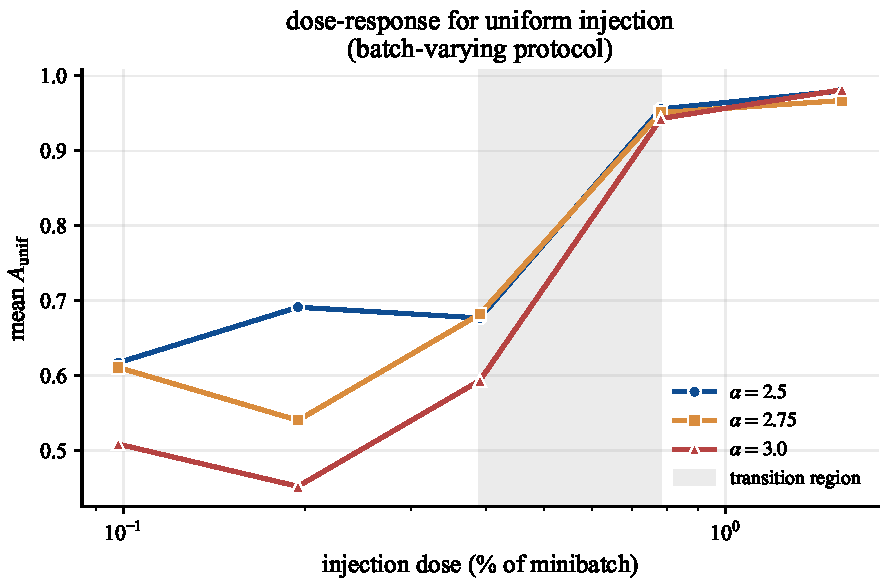
\includegraphics[width=0.7\textwidth]{fig3_doseresponse.pdf}
\caption{Dose-response curves for uniform injection at $\lambda=0.3$, three skew values (batch-varying protocol). The shaded band marks the transition region.}
\label{fig:doseresponse}
\end{figure}

\begin{table}[t]
\centering
\caption{Deconfounded dose sweep: batch size (128) and step count ($60{,}000$) fixed throughout; expected dose $q/128$ implemented by probabilistic single-slot replacement. Pooled across $\alpha\in\{2.5,2.75,3.0\}$, 24 seeds per dose point (per-$\alpha$ breakdown in Appendix~C, Table~\ref{tab:doseclean-peralpha}).}
\label{tab:doseclean}
\begin{tabular}{lccc}
\toprule
$q$ & Expected dose & Fraction generalizing & Mean $A_{\mathrm{unif}}$ \\
\midrule
0.10 & $0.078\%$ & $0/24$ & $0.478$ \\
0.25 & $0.195\%$ & $0/24$ & $0.683$ \\
0.50 & $0.391\%$ & $7/24$ & $0.846$ \\
0.75 & $0.586\%$ & $19/24$ & $0.927$ \\
1.00 & $0.781\%$ & $17/24$ & $0.924$ \\
\bottomrule
\end{tabular}
\end{table}

Three controls, matched for injected sample count at $\alpha=2.5$, $\lambda=0.3$, rank what about the injected examples matters. Each minibatch of 128 replaces $k$ of its 128 slots (not adds $k$ extra) with the intervention condition, so a dose of $k=1$ is $p=1/128\approx0.78\%$ of a fixed-size batch. The underlying skewed distribution $P_\alpha$ already assigns positive probability to every state, so what the three controls vary is not presence versus absence of support but how broadly the injected slot itself is drawn: from the same head-concentrated distribution as the rest of the batch, from a small targeted set of rare-but-short states (states with carry-chain length $c(x)<n/2$, restricted to the $N/10$ such states with the lowest $P_\alpha$ weight, i.e.\ excluding the bottleneck states with $c(x)\ge n/2$), or uniformly across the entire state space. Injecting one slot drawn from the \emph{same} skewed distribution as the rest of the batch fails to rescue (mean uniform accuracy $0.282$, close to the zero-injection baseline, consistent with this control being a null resampling of the same distribution rather than a change to the batch's composition). Injecting one slot drawn from the small targeted set of states that are rare under the skew but have short carry chains achieves partial credit (mean $0.750$) without reaching the generalization threshold in any of eight seeds. Only injection drawn uniformly across the full state space achieves complete rescue (mean $0.956$). Among these three tested distributions, uniform full-state injection is the one that rescues; a same-distribution replacement slot and a small targeted rare-but-unstructured set are both insufficient. This ranking alone conflates breadth, entropy, and state composition---all of which differ between uniform injection and the targeted set. Appendix~D decomposes breadth from composition by holding bottleneck-state exclusion fixed (bottleneck states are never in the injection pool) and varying only pool breadth among the remaining non-bottleneck states: generalization rises monotonically with pool size and reaches complete rescue by $600$ of the $992$ non-bottleneck states, matching full-state uniform injection's mean accuracy without ever including a bottleneck state. Breadth among non-bottleneck states is therefore sufficient for rescue at this cell; the partial credit of the $102$-state rare-but-short-carry pool reflects insufficient breadth rather than the absence of bottleneck states. This does not further decompose breadth from entropy, since a larger pool of non-bottleneck states also has higher entropy; we leave that finer distinction to future work. The same rescue succeeds with as few as $15{,}000$ injected samples at a shortened $15{,}000$-step budget, indicating the effect operates quickly rather than through slow accumulation. At a higher dose ($k=2$ per 128, $p{\approx}1.56\%$) under the original batch-varying protocol, all eight seeds generalize at every tested $\alpha$, consistent with the deconfounded sweep's plateau beyond $q=0.75$ rather than a renewed rise.

\subsection{Boundary shape: family discrimination}
\label{sec:results-family}

We compared five single-scale candidate functions of $\alpha$ against the measured weight-decay ceiling: $E_\alpha[c]=\sum_x P_\alpha(x)\,c(x)$, where $c(x)$ is the trailing-ones count of $x$'s binary representation (the number of low-order bits that must ripple-carry when incrementing $x$; $c(2^n-1)=n$), the same quantity that defines the ``tail''/``rare-but-short-carry'' injection pools in \S\ref{sec:results-rescue}, taken in expectation under the skew (expected carry-chain length), $2^{-\alpha}$ (pure exponential), $H_{\mathrm{lo}}=\sum_{x\ge N/2}P_\alpha(x)$ and $H_{\mathrm{tail10}}=\sum_{x\ge 9N/10}P_\alpha(x)$ (tail population mass at two thresholds), and $p_\star=P_\alpha(N-1)$ (the single rarest state's probability), where $N=2^n$. Each candidate is fit as ceiling$(\alpha)\approx C\cdot f(\alpha)$ with a single scale constant $C$ chosen by least squares in log space over the eight originally-measured $\alpha$ values ($\alpha\in\{1.5,2.0,2.1,2.25,2.4,2.5,2.6,2.7\}$), then evaluated, with $C$ frozen, at eight pre-specified held-out $\alpha$ values. At three of the eight ($\alpha=1.7$, $1.9$, $2.65$), the tested weight-decay grid at that $\alpha$ does not bracket the $0.9$ threshold---all three sampled $\lambda$ give $A_{\mathrm{unif}}$ above threshold at $\alpha=1.7$ and $1.9$, and all three give $A_{\mathrm{unif}}$ below threshold at $\alpha=2.65$---so the ceiling lies outside the tested range and is not interpolable; we report the remaining five as resolved comparisons (Table~\ref{tab:heldout}) rather than extrapolate beyond measured $\lambda$. On these five, the two best-performing candidates---expected carry-chain length $E_\alpha[c]$ and the pure exponential $2^{-\alpha}$---achieve mean prediction error of $15\%$ and $18\%$ respectively (maximum error $27\%$ and $33\%$), both smaller than either candidate's in-sample fitting error on the original eight-point grid. $E_\alpha[c]$ has the lower error at four of the five held-out points, but by a small margin at every point (absolute error difference $\le 7.4$ percentage points), so we do not read this as a clear win for one candidate over the other. The three remaining candidates ($H_{\mathrm{lo}}$, $H_{\mathrm{tail10}}$, $p_\star$) diverge sharply from the measured ceilings at these held-out points (e.g.\ $H_{\mathrm{lo}}$ predicts $0.533$ against a measured $0.155$ at $\alpha=2.05$); $p_\star$, the pre-specified bottleneck-state candidate, has the largest error, $20.5\times$ that of the best candidate. We read this as validating a single-scale model class for the boundary's shape, without resolving a unique governing law.

\begin{table}[t]
\centering
\caption{Pre-specified held-out predictions vs.\ measured ceilings at the 5 of 8 $\alpha$ values whose tested weight-decay grid brackets the $0.9$ threshold (interpolable); the remaining 3 ($\alpha=1.7,1.9,2.65$) fall outside their tested $\lambda$ range and are not resolved here.}
\label{tab:heldout}
\begin{tabular}{lccc}
\toprule
$\alpha$ & $E_\alpha[c]$ prediction & $2^{-\alpha}$ prediction & Measured ceiling \\
\midrule
2.05 & 0.173 & 0.168 & 0.155 \\
2.15 & 0.158 & 0.156 & 0.167 \\
2.35 & 0.133 & 0.136 & 0.126 \\
2.45 & 0.122 & 0.127 & 0.096 \\
2.55 & 0.112 & 0.119 & 0.089 \\
\bottomrule
\end{tabular}
\end{table}

\subsection{Local robustness and task transfer}
\label{sec:results-robustness}

We pre-specified, before running the corresponding experiments, the direction in which seven single-factor perturbations should move mean accuracy at two boundary-adjacent cells relative to the $d{=}64$, lr$=10^{-3}$, 2-layer, AdamW baseline of \S3.1 (baseline mean accuracy $0.974$ at $\alpha{=}2.5,\lambda{=}0.085$ and $0.853$ at $\alpha{=}2.25,\lambda{=}0.125$): width $d{=}32$ harder and $d{=}128$ easier; learning rate $5\times10^{-4}$ easier and $2\times10^{-3}$ harder; depth 1 layer harder and 3 layers easier; and switching from AdamW to SGD with momentum $0.9$, at otherwise unchanged hyperparameters, was predicted to perform substantially worse, following the literature on adaptive optimizers' role in grokking. Two further cells ($d{=}32$,lr$=5\times10^{-4}$ and $d{=}128$,lr$=2\times10^{-3}$) test whether the width and learning-rate effects combine additively, with no directional prediction attached. A perturbation counts as confirmed if mean accuracy moves in the predicted direction at both cells (Table~\ref{tab:robustness}). Four of the seven directional predictions are confirmed at both cells: width $d{=}32$ (harder), learning rate $2\times10^{-3}$ (harder), depth 1 layer (harder), and SGD with momentum (substantially worse, mean $0.001$ against the AdamW baseline). Width $d{=}128$ and learning rate $5\times10^{-4}$ (both predicted easier) are confirmed only at $\alpha{=}2.25,\lambda{=}0.125$; at $\alpha{=}2.5,\lambda{=}0.085$, the baseline is already within a few points of the $0.9$-threshold ceiling (mean $0.974$), leaving little room to move further in the easier direction, and both show a small mean decrease there instead. Depth 3 layers (predicted easier) is confirmed at neither cell: mean accuracy is essentially unchanged at the first cell and falls at the second. Because SGD with momentum was not independently tuned, we read its result as evidence that the effect is not optimizer-invariant, rather than as a controlled ranking of optimizers.

\begin{table}[t]
\centering
\small
\caption{Pre-specified directional predictions and outcomes at two boundary-adjacent cells ($\alpha{=}2.5,\lambda{=}0.085$, baseline mean $0.974$; and $\alpha{=}2.25,\lambda{=}0.125$, baseline mean $0.853$), 5 seeds each. Confirmation criterion: mean accuracy moves in the predicted direction at both cells. Four of seven directional predictions confirmed at both cells; the two interaction cells test additivity and carry no direction.}
\label{tab:robustness}
\begin{tabular}{@{}p{3.3cm}p{2.3cm}p{2.7cm}p{2.6cm}@{}}
\toprule
Perturbation & Predicted direction & Mean accuracy (both cells) & Outcome \\
\midrule
Width $d{=}32$ & harder & $0.384$, $0.357$ & confirmed \\
Width $d{=}128$ & easier & $0.951$, $0.992$ & confirmed at cell 2 only \\
Learning rate $5\times10^{-4}$ & easier & $0.970$, $0.979$ & confirmed at cell 2 only \\
Learning rate $2\times10^{-3}$ & harder & $0.845$, $0.813$ & confirmed \\
Depth 1 layer & harder & $0.731$, $0.828$ & confirmed \\
Depth 3 layers & easier & $0.974$, $0.807$ & not confirmed \\
$d{=}32$, lr$=5\times10^{-4}$ (interaction) & no direction (additivity test) & $0.444$, $0.623$ & width dominates \\
$d{=}128$, lr$=2\times10^{-3}$ (interaction) & no direction (additivity test) & $0.930$, $0.931$ & width dominates \\
SGD, momentum $0.9$ & substantially worse & $0.001$, $0.001$ & confirmed \\
\bottomrule
\end{tabular}
\end{table}

\subsection{Transfer to modular addition}
\label{sec:results-modadd}

We repeated the injection comparison from \S\ref{sec:results-rescue} on modular addition ($p=97$), at its own clean failure region ($\alpha=3.0$, $\lambda=0.3$), with the same dose ($k=1$ per batch of 128) and the same architecture, optimizer, and evaluation convention (\S3.5). At this second task, ``rare-but-short'' and ``head-concentrated'' states are not defined by carry length, so the two targeted controls are the natural analogues here: rare, large-operand states, and the most frequent states. The zero-injection baseline at this cell is $0.413$ mean accuracy (0/3 generalizing). The ranking direction reproduces: uniform injection achieves $0.934$ mean accuracy with three of five seeds generalizing; injection restricted to rare, large-operand states achieves $0.721$ with zero of five generalizing; injection restricted to the most frequent states achieves $0.396$ with zero of five generalizing, close to the zero-injection baseline (Figure~\ref{fig:modadd}). This reproduces the injection-ranking direction under sample-count-matched controls on a second arithmetic task; the partial 3/5 rate for uniform injection here is weaker than LARGECOUNTER's 8/8, so we read this as ranking transfer rather than a matched-magnitude replication.

\begin{figure}[t]
\centering
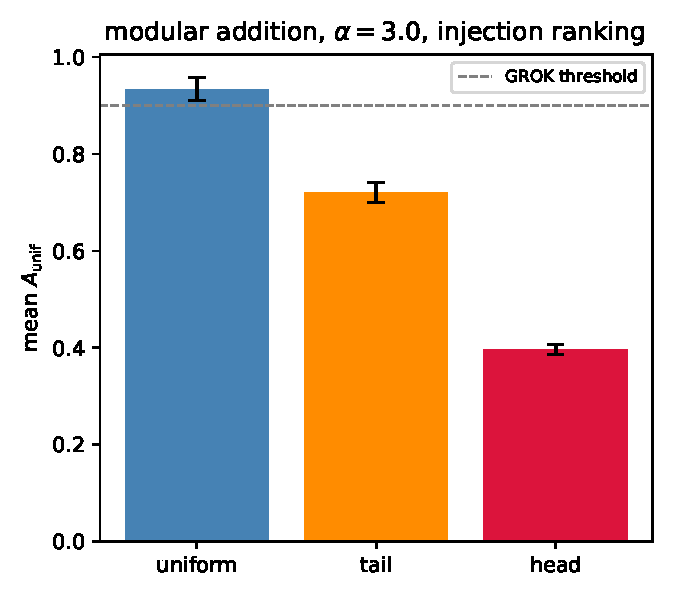
\includegraphics[width=0.45\textwidth]{fig4_modadd.pdf}
\caption{Injection ranking on modular addition, $\alpha=3.0$, $\lambda=0.3$, $k=1$. Error bars are s.e.m. over 5 seeds.}
\label{fig:modadd}
\end{figure}

\subsection{A stress test: Dyck-1 forced-position prediction}
\label{sec:results-dyck}

Modular addition is closely related to LARGECOUNTER in structure. We additionally probed a non-arithmetic task---Dyck-1 forced-position prediction (\S3.5), skewed by each valid path's maximum nesting depth---as a deliberately harder, out-of-domain test of how far the injection ranking travels. Across a formal boundary grid (540 runs, ten seeds per cell), a two-dimensional failure region again emerges as both skew and weight decay increase, and its deepest cells collapse to a fixed, degenerate accuracy value reproduced identically across independent seeds, including a seed never previously run (Figure~\ref{fig:dyckboundary}).

\begin{figure}[t]
\centering
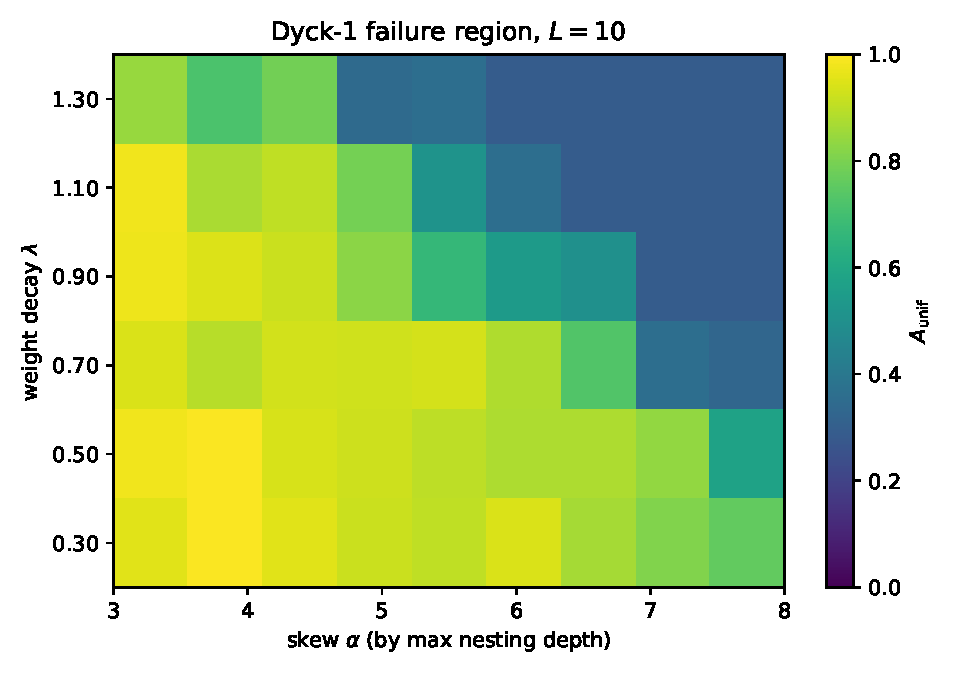
\includegraphics[width=0.75\textwidth]{fig5_dyckboundary.pdf}
\caption{Dyck-1 formal boundary grid, $L=10$, 540 runs, ten seeds per cell.}
\label{fig:dyckboundary}
\end{figure}

Rescue is directionally but not completely successful here. At a deep-collapse cell, the same uniform-injection intervention that fully rescues the other two tasks improves accuracy only partially (mean $0.398$, zero of five seeds reaching the generalization threshold), while targeted and frequent-state injection remain at the collapsed baseline (both $0.289$)---the injection-ranking direction reproduces, but the magnitude does not. At one boundary cell, extending training from 60{,}000 to 240{,}000 steps changes the outcome from two-of-three generalizing to zero-of-three: examining the full accuracy trajectories (Figure~\ref{fig:dycktrajectory}) shows this is not training becoming harmful, but a shorter run stopping inside a metastable high-accuracy plateau that the longer run continues past into a collapse, consistent with independently-reported anti-grokking dynamics in which test accuracy collapses back to chance after a network has already generalized \citep{prakash2026antigrokking,prakash2026longhorizon}.

\begin{figure}[t]
\centering
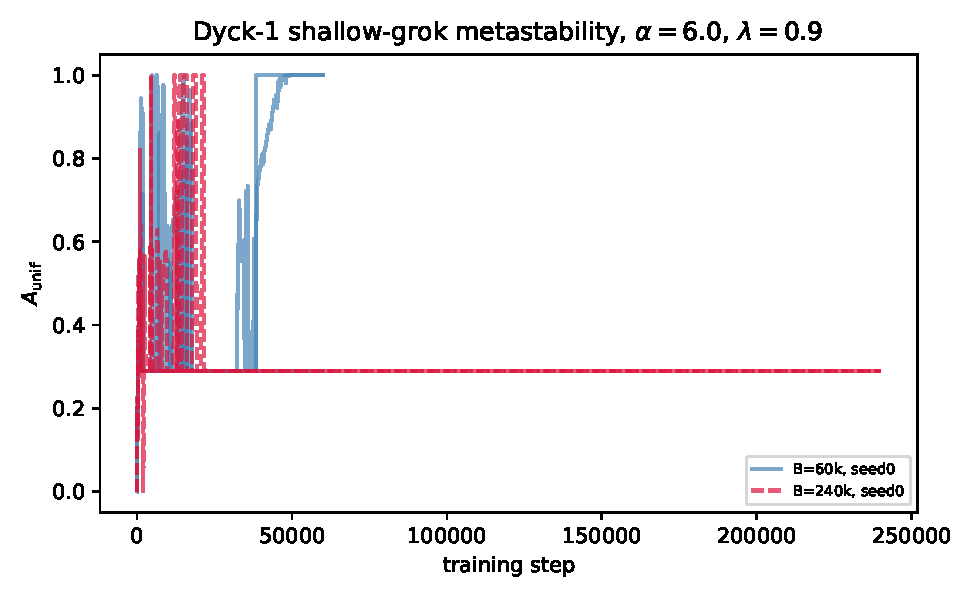
\includegraphics[width=0.75\textwidth]{fig6_dycktrajectory.pdf}
\caption{Full accuracy trajectories at $\alpha=6.0$, $\lambda=0.9$: 60k-step runs (solid) that stop inside the metastable plateau vs.\ 240k-step runs (dashed) on the same configuration that continue past it into collapse.}
\label{fig:dycktrajectory}
\end{figure}

Dyck-1 therefore qualifies the transfer claim precisely: the failure topology and the direction of the injection ranking transfer to a non-arithmetic task, while complete rescue and budget-monotonic behavior do not. Full boundary and rescue data appear in Appendix~B; full accuracy trajectories underlying the metastable-plateau finding appear in Figure~\ref{fig:dycktrajectory} above.

\section{Discussion}

The corrected direction of the weight-decay ceiling---falling, rather than rising, with skew---and the refutation of a targeted-rarity rescue curriculum in favor of broadening the injected examples' exposure across the state space (\S\ref{sec:results-rescue}) both depart from an earlier proposal that predicted the opposite in each case. Both corrections came from running the experiment, not from refining the theory in advance; we read this as the value of the empirical approach we take here, not as an incidental finding to note in passing.

Table~\ref{tab:relatedwork} summarizes how the nearest prior work compares to this paper's contributions along the axes of skew, finite-budget mapping, rescue controls, exposure matching, task transfer, and scale.

\begin{table}[t]
\centering
\footnotesize
\caption{Comparison to the nearest prior work along the axes this paper contributes.}
\label{tab:relatedwork}
\begin{tabular}{@{}p{2.6cm}p{1.9cm}cccc>{\centering\arraybackslash}p{1.1cm}@{}}
\toprule
Work & Skew axis & \shortstack{Finite-\\budget map} & \shortstack{Rescue\\controls} & \shortstack{Exposure\\match} & \shortstack{Task\\transfer} & Toy scale \\
\midrule
Zhao \citeyearpar{zhao2026grok} & discrete (2 pts) & --- & --- & --- & --- & \checkmark \\
Liu et al.\ \citeyearpar{liu2022effectivetheory,liu2022omnigrok} & data fraction & \checkmark & --- & --- & \checkmark & \checkmark \\
Singh et al.\ \citeyearpar{singh2025datafallsshort} & data quantity & --- & \checkmark (KD) & --- & --- & \checkmark \\
Bi et al.\ \citeyearpar{bi2026falsifiable} & group order & \checkmark (critical) & --- & --- & --- & \checkmark \\
This paper & continuous $\alpha$ & \checkmark & \checkmark (ranked) & \checkmark & \checkmark (2 tasks) & \checkmark \\
\bottomrule
\end{tabular}
\end{table}

\subsection{Limitations}
All results in this paper are established at $n\le 12$, $d\le 128$, within a single decoder-only Transformer architecture family. The family-discrimination analysis in \S\ref{sec:results-family} establishes a model class, not a closed-form law: the two best-performing candidates differ by a small margin at every held-out point. The robustness study (\S\ref{sec:results-robustness}) confirms 4 of 7 directional predictions, and the injection ranking (\S\ref{sec:results-rescue}, Appendix~D) shows breadth among non-bottleneck states is sufficient for rescue, but does not further decompose breadth from entropy.

\section{Conclusion}

We map grokkability across a continuous data-skew axis and weight decay on an autoregressive counting task, find a two-regime failure structure that persists at a second problem size, and identify a minimal intervention---uniform full-state injection, ranked against sample-count and targeted-rarity alternatives---that rescues both of its failure modes. The same ranking transfers to a second arithmetic task under sample-count-matched controls, and a third, non-arithmetic task shows us precisely where that transfer holds and where it does not.

\subsection*{Code and data availability}
All training code, the frozen verdict rule, per-seed result logs, and the pre-specified prediction files (Tables~\ref{tab:heldout} and \ref{tab:robustness}, recorded before the corresponding measurement runs per \S3.7) are available at \url{https://github.com/yangyangtiaoguo/grokking}.

\bibliographystyle{plainnat}
\bibliography{references}

\appendix

\section{Per-cell seed counts, $(\alpha,\lambda)$ phase diagram}
\label{app:seedcounts}
Table~\ref{tab:appendixseeds} gives the number of distinct $\lambda$ points and the seed-count range at each $\alpha$ underlying Figure~\ref{fig:phasediagram}'s ceiling curve (60{,}000-step budget, $n=10$). Cells near a resolved ceiling were sampled at up to 10 seeds; exploratory cells away from the boundary used 3.

\begin{table}[h]
\centering
\small
\caption{Per-$\alpha$ grid density and seed-count range, $n=10$, 60k-step budget.}
\label{tab:appendixseeds}
\begin{tabular}{lccc}
\toprule
$\alpha$ & \# $\lambda$ points & Min seeds/cell & Max seeds/cell \\
\midrule
0.0 & 6 & 3 & 3 \\
1.0 & 8 & 3 & 3 \\
1.5 & 3 & 3 & 3 \\
2.0 & 11 & 3 & 5 \\
2.1 & 7 & 3 & 5 \\
2.25 & 11 & 3 & 5 \\
2.4 & 9 & 3 & 5 \\
2.5 & 11 & 3 & 5 \\
2.6 & 9 & 3 & 5 \\
2.7 & 3 & 5 & 5 \\
2.75 & 13 & 3 & 10 \\
2.9 & 6 & 3 & 8 \\
3.0 & 9 & 3 & 6 \\
\bottomrule
\end{tabular}
\end{table}

\section{Dyck-1 formal boundary grid and rescue data}
\label{app:dyck}
Table~\ref{tab:dyckboundary} gives the full $(\alpha,\lambda)$ mean $A_{\mathrm{unif}}$ grid underlying Figure~\ref{fig:dyckboundary} (10 seeds per cell, 540 runs total). Table~\ref{tab:dyckrescue} gives the injection-ranking means underlying \S\ref{sec:results-dyck}'s rescue comparison at the deep-collapse cell $\alpha=5.5$, $\lambda=1.3$.

\begin{table}[h]
\centering
\small
\caption{Dyck-1 formal boundary grid: mean $A_{\mathrm{unif}}$, $L=10$, 10 seeds/cell.}
\label{tab:dyckboundary}
\begin{tabular}{lcccccc}
\toprule
$\alpha$ & $\lambda{=}0.3$ & $0.5$ & $0.7$ & $0.9$ & $1.1$ & $1.3$ \\
\midrule
3.0 & 0.96 & 0.98 & 0.94 & 0.97 & 0.98 & 0.85 \\
3.5 & 1.00 & 0.99 & 0.89 & 0.95 & 0.87 & 0.71 \\
4.0 & 0.95 & 0.94 & 0.93 & 0.92 & 0.90 & 0.79 \\
4.5 & 0.92 & 0.92 & 0.93 & 0.83 & 0.79 & 0.34 \\
5.0 & 0.90 & 0.90 & 0.93 & 0.67 & 0.51 & 0.36 \\
5.5 & 0.94 & 0.88 & 0.88 & 0.55 & 0.36 & 0.29 \\
6.0 & 0.86 & 0.88 & 0.73 & 0.50 & 0.29 & 0.29 \\
7.0 & 0.81 & 0.84 & 0.36 & 0.29 & 0.29 & 0.29 \\
8.0 & 0.76 & 0.58 & 0.33 & 0.29 & 0.29 & 0.29 \\
\bottomrule
\end{tabular}
\end{table}

\begin{table}[h]
\centering
\small
\caption{Dyck-1 injection ranking at the deep-collapse cell ($\alpha=5.5$, $\lambda=1.3$), $k=1$ per batch of 128.}
\label{tab:dyckrescue}
\begin{tabular}{lccc}
\toprule
Injection & Mean $A_{\mathrm{unif}}$ & Seeds at threshold & $n$ \\
\midrule
none ($k=0$) & 0.289 & 0/3 & 3 \\
head & 0.289 & 0/5 & 5 \\
tail & 0.289 & 0/5 & 5 \\
uniform & 0.398 & 0/5 & 5 \\
\bottomrule
\end{tabular}
\end{table}

\section{Per-$\alpha$ breakdown of the deconfounded dose sweep}
\label{app:doseclean}
Table~\ref{tab:doseclean} pools 24 seeds per dose point across three $\alpha$ values; Table~\ref{tab:doseclean-peralpha} gives the same sweep broken out per $\alpha$ (8 seeds/cell).

\begin{table}[h]
\centering
\small
\caption{Deconfounded dose sweep by $\alpha$: fraction generalizing / mean $A_{\mathrm{unif}}$, 8 seeds/cell.}
\label{tab:doseclean-peralpha}
\begin{tabular}{lccccc}
\toprule
$\alpha$ & $q{=}0.10$ & $q{=}0.25$ & $q{=}0.50$ & $q{=}0.75$ & $q{=}1.00$ \\
\midrule
2.5 & 0/8 (0.551) & 0/8 (0.725) & 3/8 (0.886) & 7/8 (0.942) & 7/8 (0.947) \\
2.75 & 0/8 (0.469) & 0/8 (0.728) & 3/8 (0.839) & 6/8 (0.922) & 5/8 (0.921) \\
3.0 & 0/8 (0.412) & 0/8 (0.594) & 1/8 (0.811) & 6/8 (0.918) & 5/8 (0.906) \\
\bottomrule
\end{tabular}
\end{table}

\section{Breadth versus composition in the injection pool}
\label{app:breadth}
The rescue comparison in \S\ref{sec:results-rescue} shows that a targeted pool of the $N/10=102$ rarest non-bottleneck states (\S3.4's rare-but-short-carry pool, excluding all bottleneck states with carry length $c(x)\ge n/2$) achieves only partial credit (mean $0.750$), while injection drawn from the full state space---which does include the 32 bottleneck states---achieves complete rescue (mean $0.956$). Because these two conditions differ in both breadth (102 vs.\ 1024 candidate states) and composition (bottleneck states excluded vs.\ included), this comparison alone cannot say which property is responsible.

We isolate breadth by holding composition fixed: bottleneck states ($c(x)\ge n/2$, 32 of 1024 states) are excluded from the injection pool at every setting, and only the pool size $K$ among the remaining 992 non-bottleneck states is varied, $K\in\{102,300,600,992\}$ (the $K$ non-bottleneck states with the lowest $P_\alpha$ weight), at the same cell as the rescue battery ($\alpha=2.5$, $\lambda=0.3$, $k=1$ per batch of 128, 8 seeds). $K=102$ reproduces the rare-but-short-carry pool exactly.

\begin{table}[h]
\centering
\caption{Breadth-only sweep with bottleneck states permanently excluded from the injection pool: fraction generalizing and mean $A_{\mathrm{unif}}$, 8 seeds/cell.}
\label{tab:breadth}
\begin{tabular}{lcc}
\toprule
$K$ (non-bottleneck pool size) & Fraction generalizing & Mean $A_{\mathrm{unif}}$ \\
\midrule
102 & 0/8 & 0.750 \\
300 & 1/8 & 0.852 \\
600 & 8/8 & 0.947 \\
992 & 7/8 & 0.949 \\
\bottomrule
\end{tabular}
\end{table}

Generalization rises monotonically with $K$ and reaches complete rescue at $K=600$, with $K=992$ (all non-bottleneck states, still excluding every bottleneck state) statistically matching full-state uniform injection's mean ($0.949$ vs.\ $0.956$). Bottleneck-state inclusion is therefore not necessary for rescue at this cell: breadth among non-bottleneck states alone is sufficient once the pool is large enough, and the partial credit of the original $K=102$ rare-but-short-carry pool reflects insufficient breadth rather than the absence of bottleneck states per se.

\end{document}
